\appendix
\chapter{Statistics} \label{ch:appendix_statistic}
\section{Statistics - can }
% remove comment if you wish to add Appendix to contentsline.
%\addcontentsline{toc}{chapter}{Appendix A: How to download ERA5 data}
%%%% MEAN
\begin{figure}[ht]
    \centering
    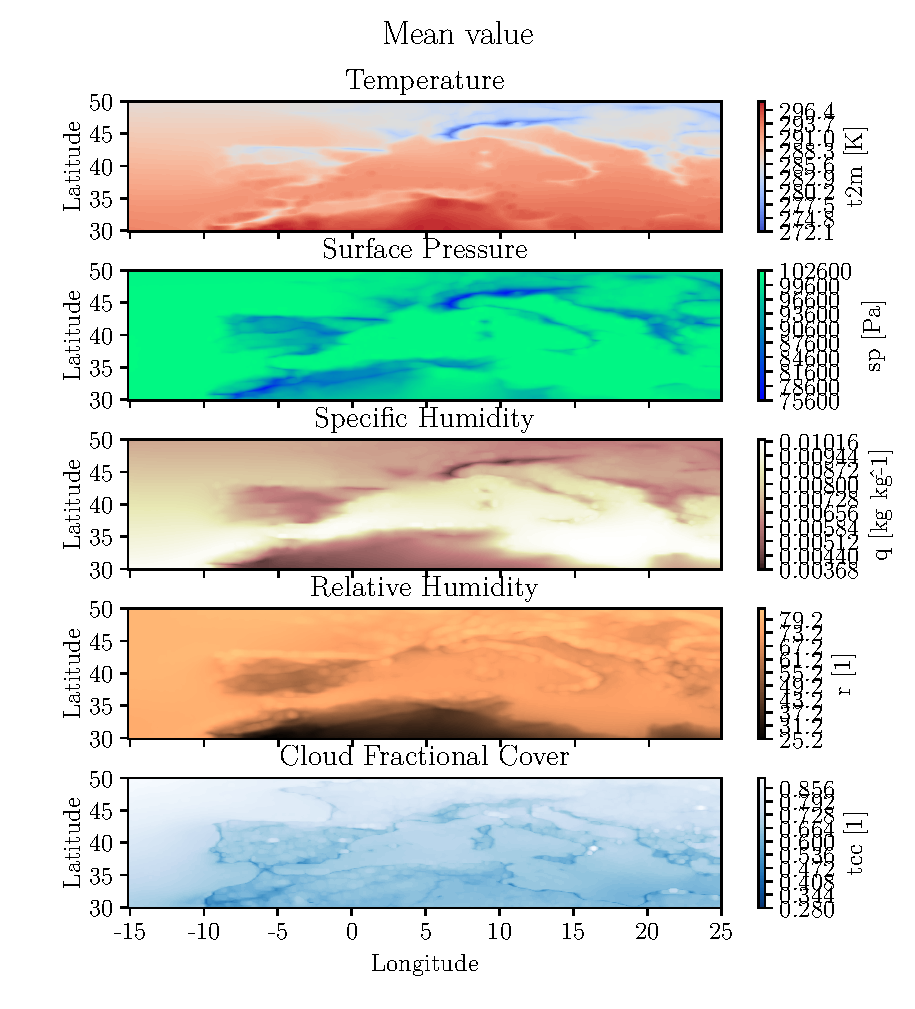
\includegraphics{python_figs/contourplot_all_variables_mean.pdf}
    \caption{Contour plot showing the local (pixel) mean of all variables.}
    \label{fig:contour_mean_all_vars}
\end{figure}

\section{Temporal statistics} \label{sec:all_stats}

%%% ALL LOCAL STATISTICS FOR VARIABLES 
%% TEMPERATURE
\begin{figure}[ht]
    \centering
    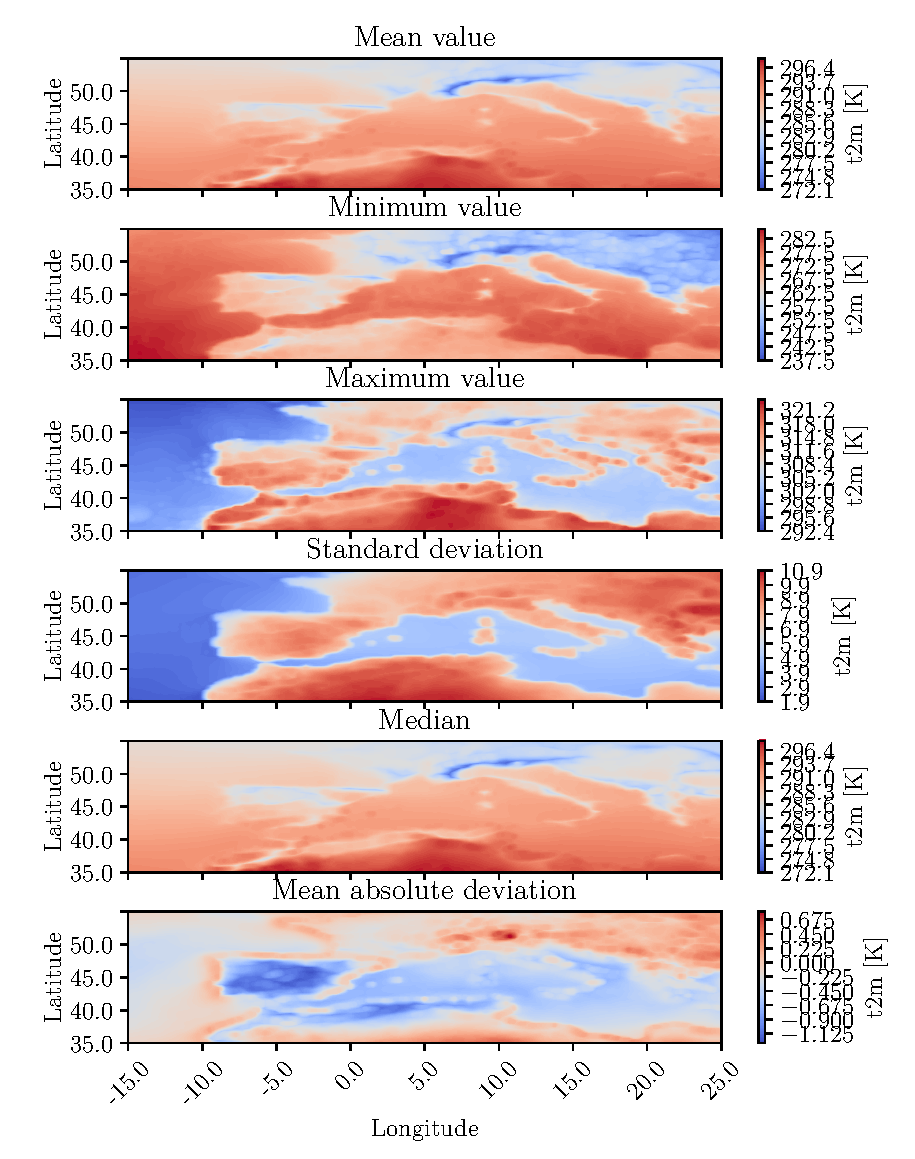
\includegraphics{python_figs/all_stat_variable_t2m.pdf}
    \caption{Contour plot showing the local (pixel) statistics for temperature.}
    \label{fig:all_stats_t2m}
\end{figure}

%% SURFACE PRESSURE 
\begin{figure}[ht]
    \centering
    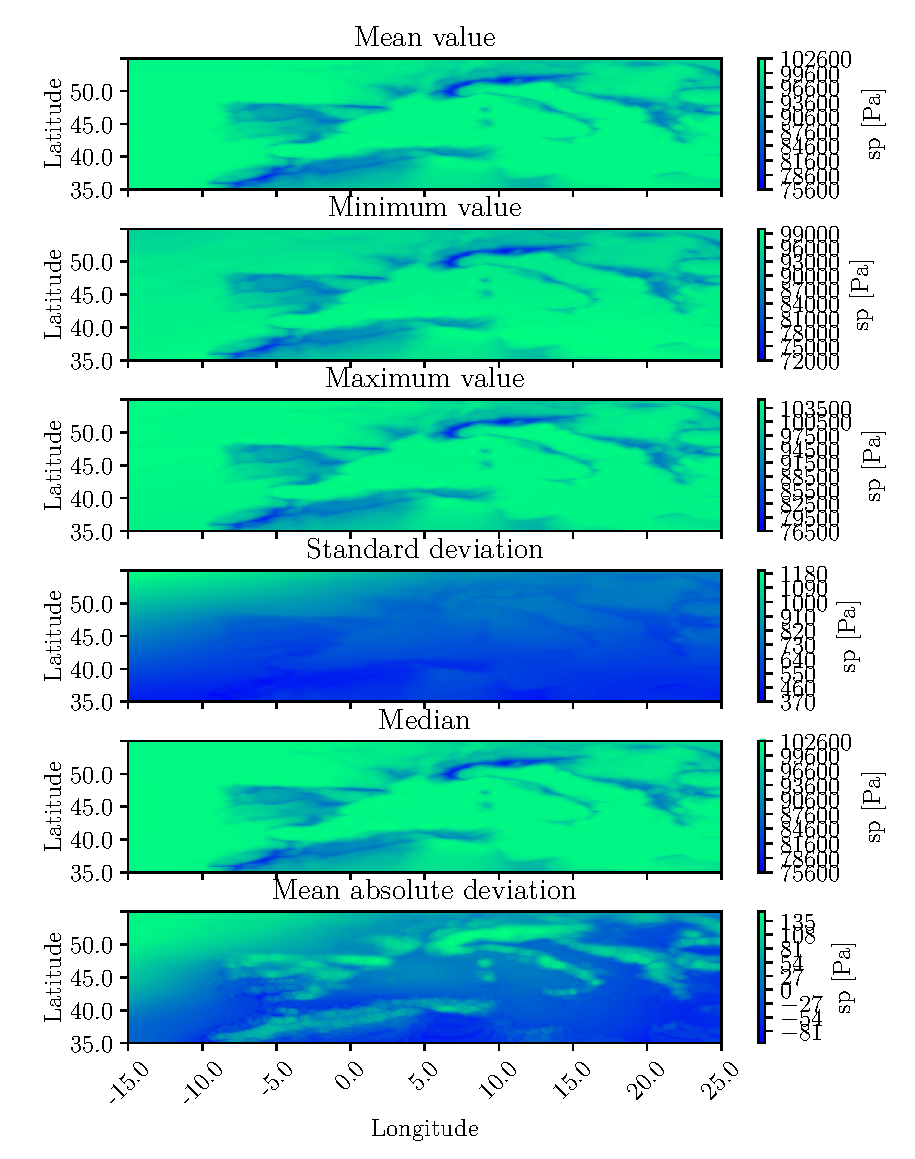
\includegraphics{python_figs/all_stat_variable_sp.pdf}
    \caption{Contour plot showing the local (pixel) statistics for surface pressure.}
    \label{fig:all_stats_sp}
\end{figure}

%% RELATIVE HUMIDITY 
\begin{figure}[ht]
    \centering
    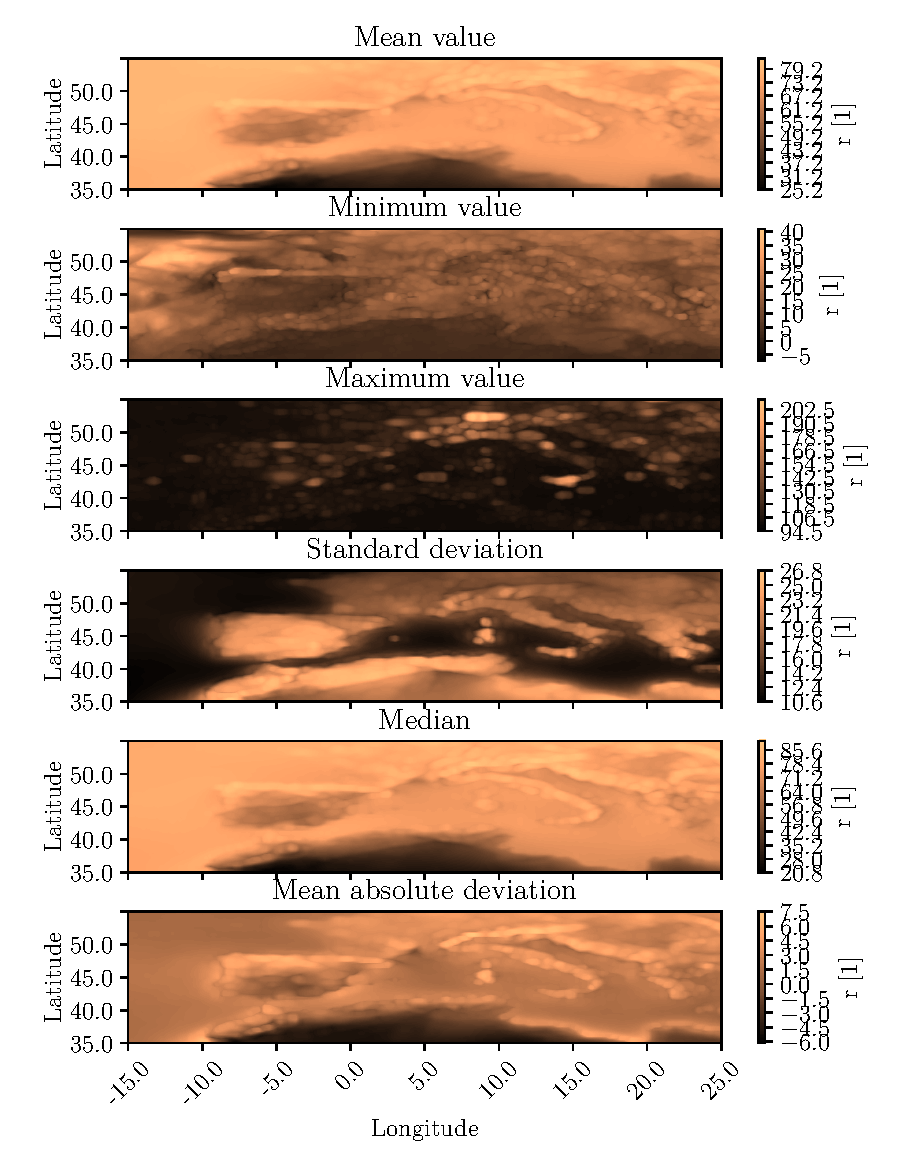
\includegraphics{python_figs/all_stat_variable_r.pdf}
    \caption{Contour plot showing the local (pixel) statistics for relative humidity.}
    \label{fig:all_stats_r}
\end{figure}


%% SPECIFIC HUMIDITY 
\begin{figure}[ht]
    \centering
    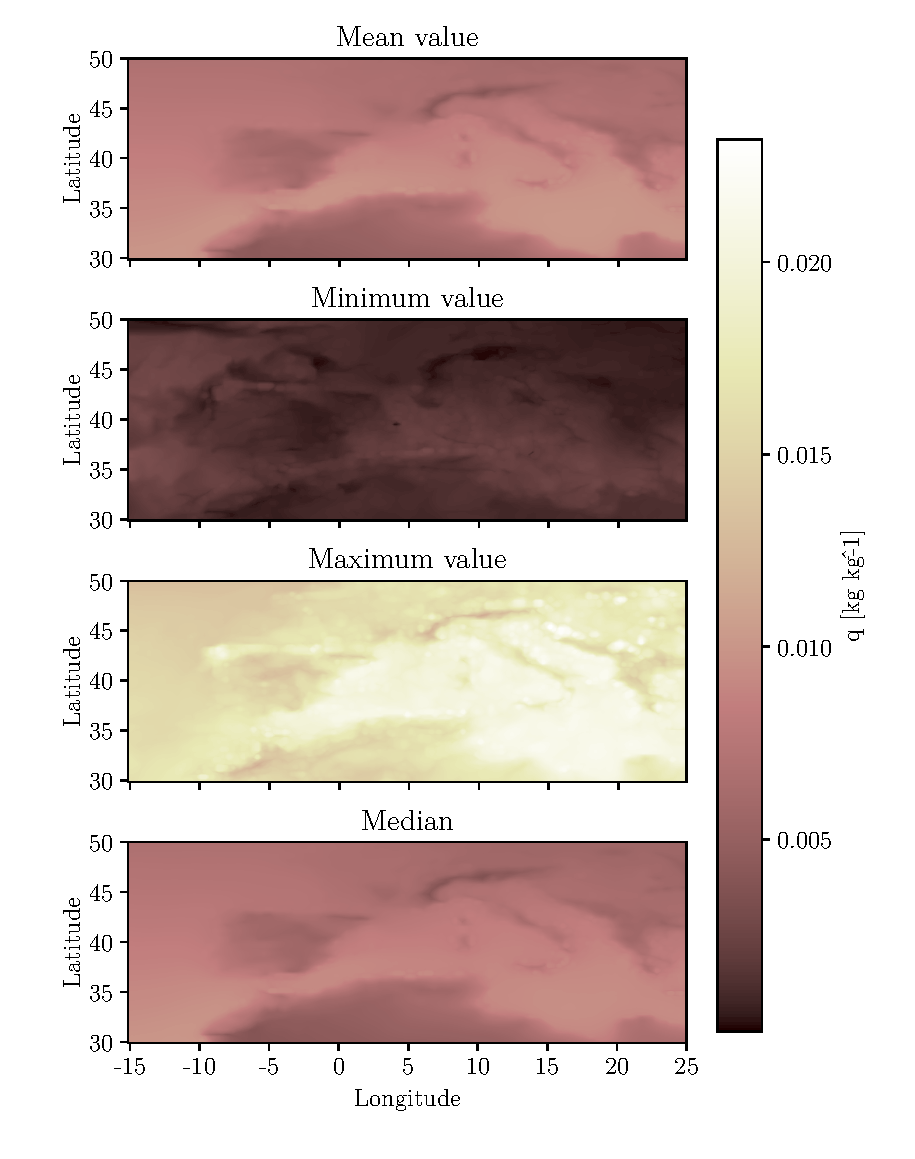
\includegraphics{python_figs/all_stat_variable_q.pdf}
    \caption{Contour plot showing the local (pixel) statistics for spesific humidity.}
    \label{fig:all_stats_q}
\end{figure}

\cleardoublepage

\chapter{Seasonal effects}
This section has more plots. 
\begin{figure}[ht]
    \centering
    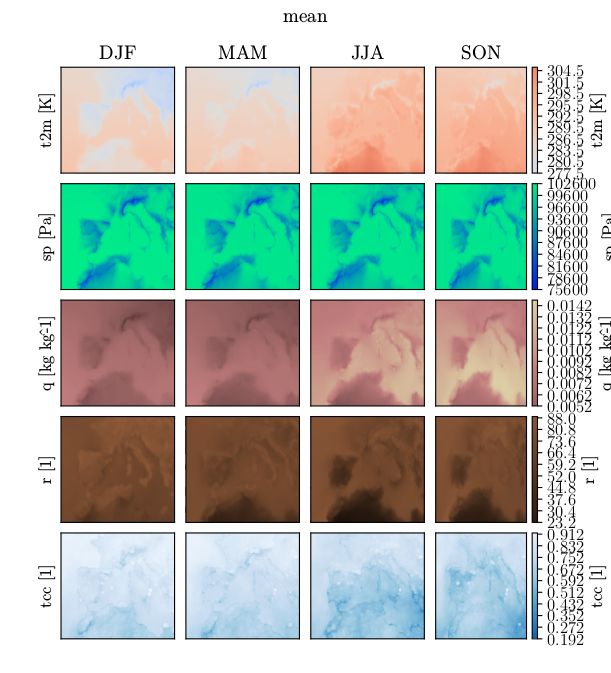
\includegraphics{python_figs/seasonal_mean_all_variables.png}
    \caption{Seasonal mean}
    \label{fig:seasonal_mean}
\end{figure}

\begin{figure}[ht]
    \centering
    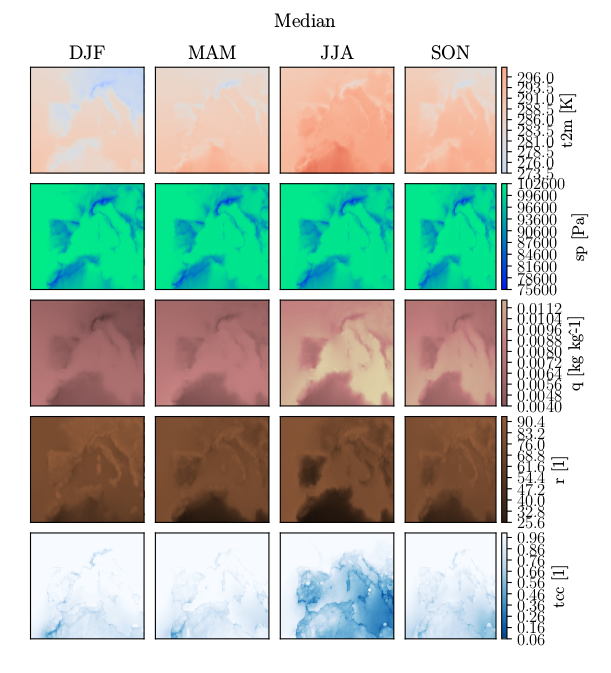
\includegraphics{python_figs/seasonal_median_all_variables.png}
    \caption{Seasonal median}
    \label{fig:seasonal_median}
\end{figure}

\chapter{Performance of other models}
Currently it show the plots that could be generated to show the performance for other model. The plots below is generated based on dummy data. 

%%%% TARGET PREDICITON HORIZONTAL
\begin{figure}[ht]
    \centering
    \includegraphics{python_figs/target_prediction_plot_horizonal.pdf}
    \caption{Comparison target and predicted cloud fractional cover.}
    \label{fig:target_predict_horizontal}
\end{figure}

%%%% TARGET PREDICITON HORIZONTAL
\begin{figure}[ht]
    \centering
    \includegraphics{python_figs/target_prediction_plot_vertical.pdf}
    \caption{Comparison target and predicted vertical cloud fractional cover.}
    \label{fig:target_predict_vertical}
\end{figure}

%%%% TARGET PREDICITON ERA5
\begin{figure}[ht]
    \centering
    \includegraphics{python_figs/target_prediction_era5_plot_horizonal.pdf}
    \caption{Comparison target, predicted and era5 horizontal cloud fractional cover.}
    \label{fig:target_predict_era5_vertical}
\end{figure}

\cleardoublepage


\chapter{Time lapse of \acrlong{cfc}. }

\begin{figure}[ht]
    \centering
    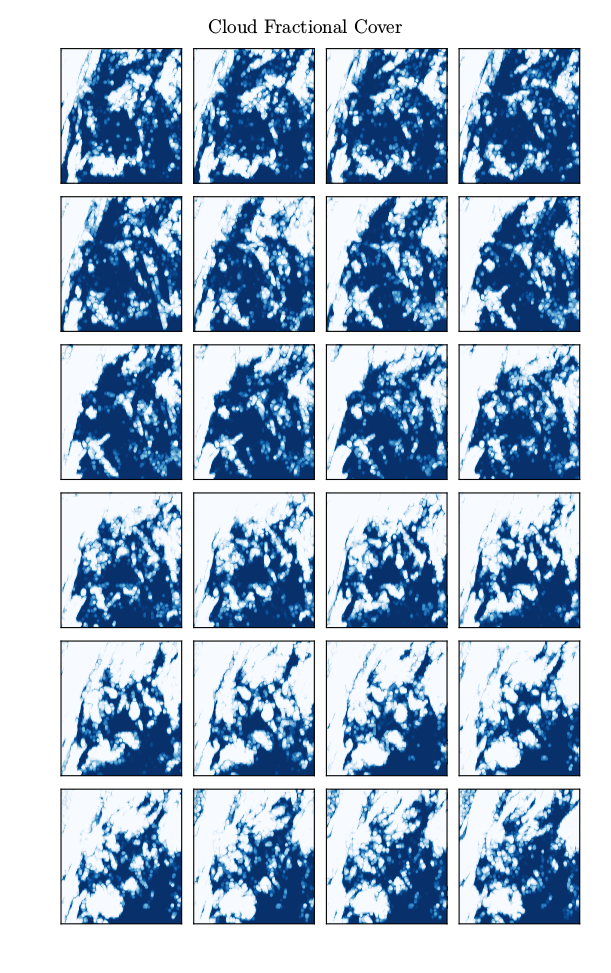
\includegraphics[scale=0.7]{python_figs/timelapse_cloud_cover_24hrs_from_2010-07-01.png}
    \caption{Time lapse photo, trying to detect the signal you would get from cloud cover within 24 hours.}
    \label{fig:time_lapse}
\end{figure}



\chapter{First week of every month in 2012}
%\addcontentsline{toc}{chapter}{Appendix D: Study 2012}

\begin{figure}[ht]
    \centering
    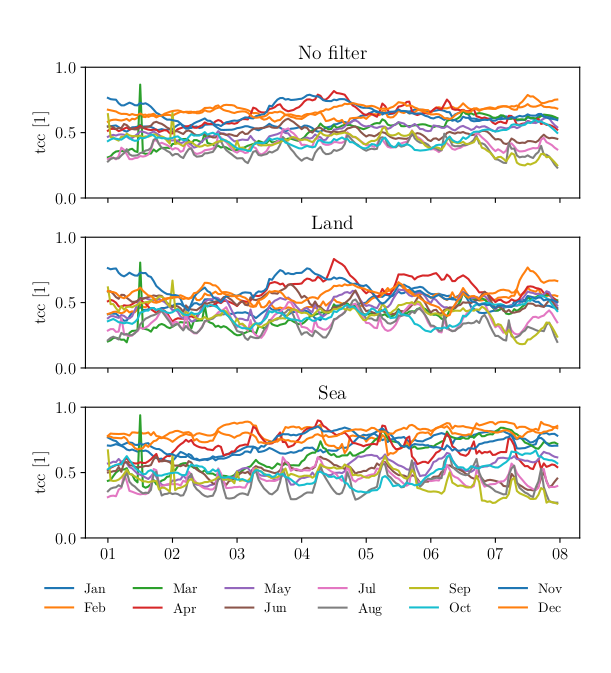
\includegraphics{python_figs/spatially_averaged_one_week_tcc_seperated_by_filters.png}
    \caption{First week of every month in 2012 merged into one figure.}
    \label{fig:all_first_week_one_figure}
\end{figure}


\begin{figure}[ht]
    \centering
    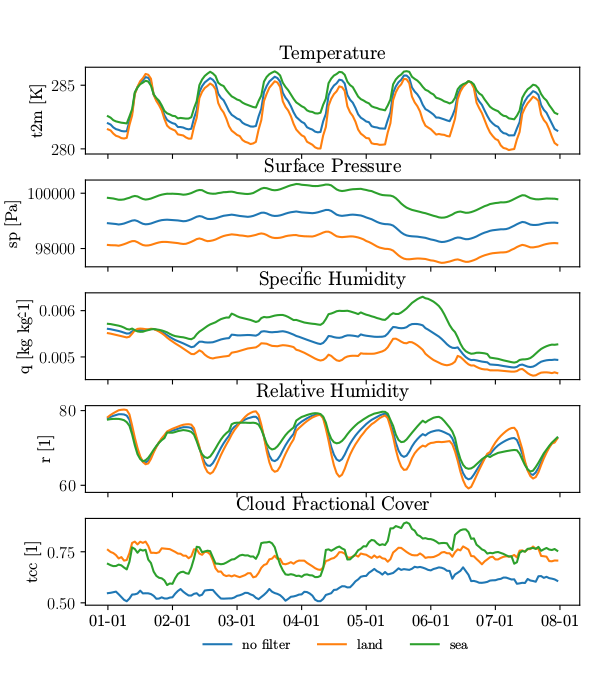
\includegraphics{python_figs/spatially_averaged_one_week_from_2012-01-01.png}
    \caption{Signal January 2012.}
    \label{fig:jan12}
\end{figure}

\begin{figure}[ht]
    \centering
    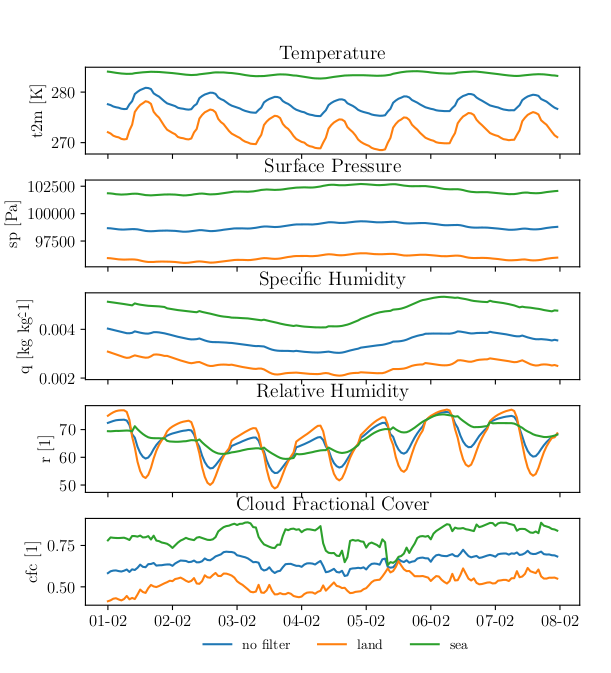
\includegraphics{python_figs/spatially_averaged_one_week_from_2012-02-01.png}
    \caption{Signal February 2012.}
    \label{fig:feb12}
\end{figure}

\begin{figure}[ht]
    \centering
    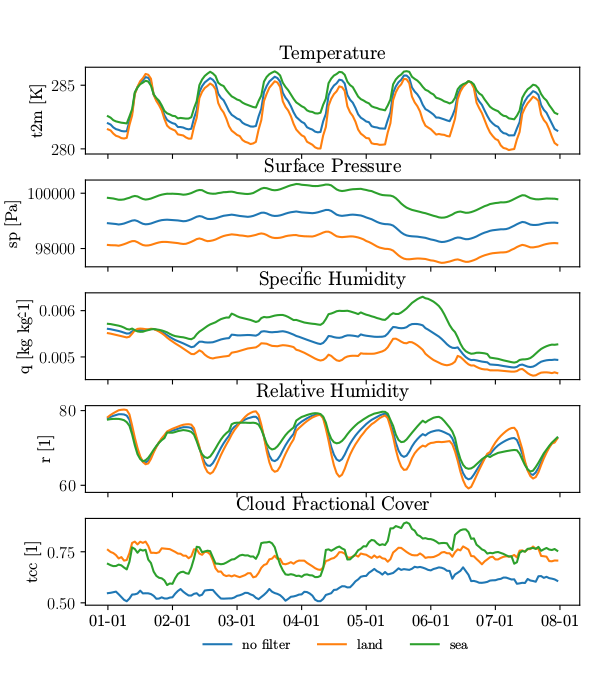
\includegraphics{python_figs/spatially_averaged_one_week_from_2012-01-01.png}
    \caption{Signal March 2012.}
    \label{fig:jan12}
\end{figure}
\begin{figure}[ht]
    \centering
    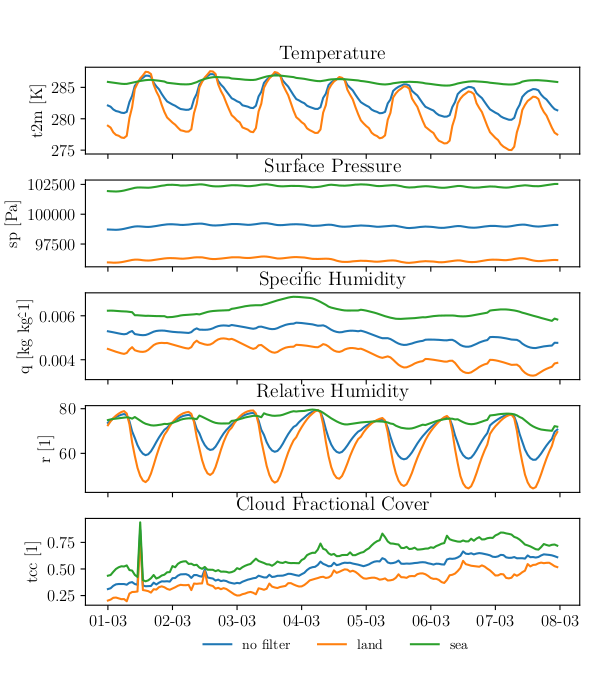
\includegraphics{python_figs/spatially_averaged_one_week_from_2012-03-01.png}
    \caption{Signal January 2012.}
    \label{fig:jan12}
\end{figure}
\begin{figure}[ht]
    \centering
    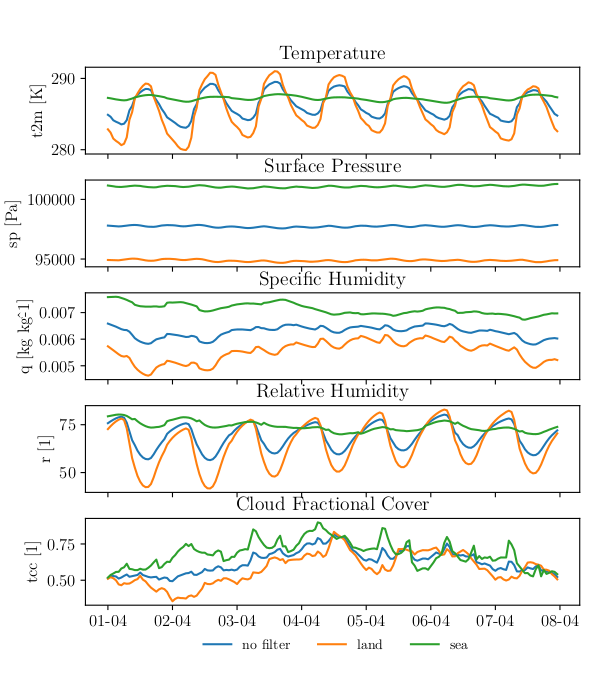
\includegraphics{python_figs/spatially_averaged_one_week_from_2012-04-01.png}
    \caption{Signal April 2012.}
    \label{fig:april12}
\end{figure}



\begin{figure}[ht]
    \centering
    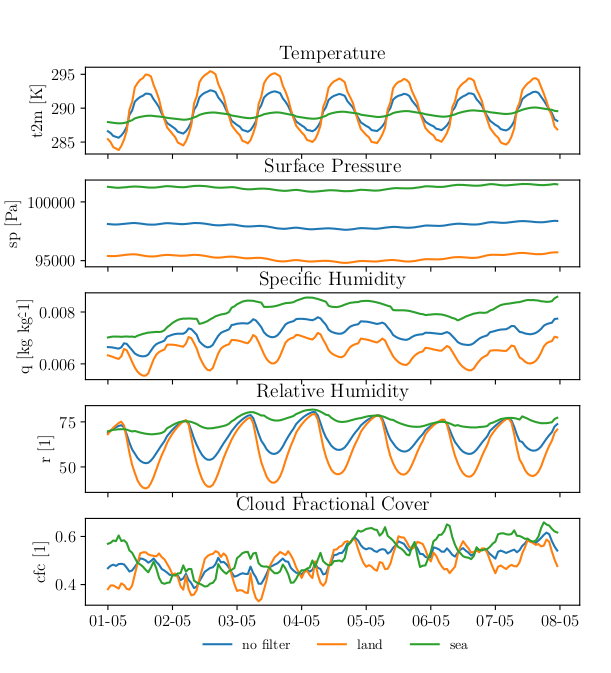
\includegraphics{python_figs/spatially_averaged_one_week_from_2012-05-01.png}
    \caption{Signal May 2012.}
    \label{fig:may12}
\end{figure}


\begin{figure}[ht]
    \centering
    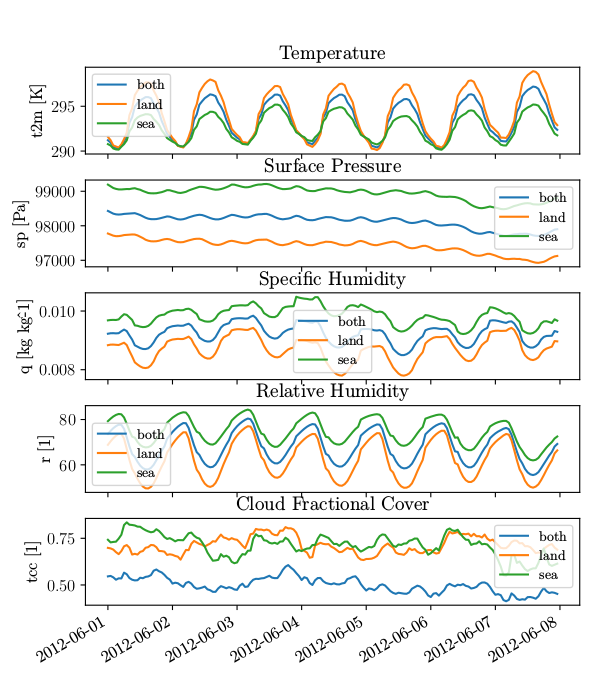
\includegraphics{python_figs/spatially_averaged_one_week_from_2012-06-01.png}
    \caption{Signal June 2012.}
    \label{fig:jun12}
\end{figure}

\begin{figure}[ht]
    \centering
    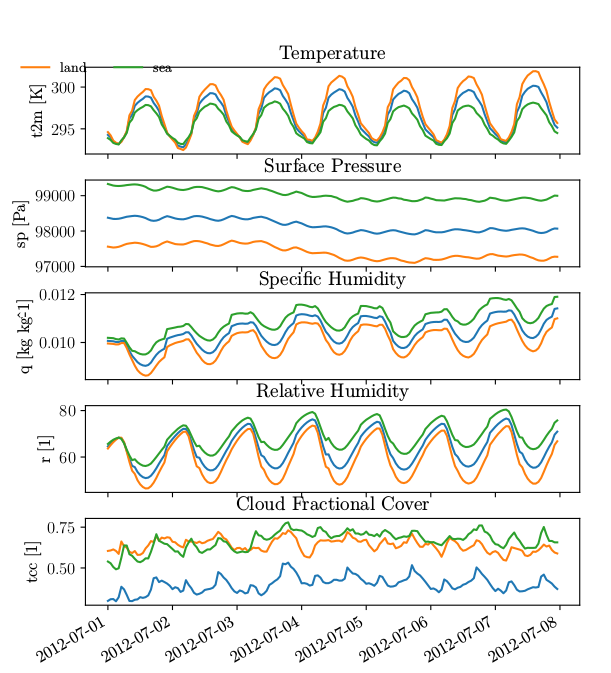
\includegraphics{python_figs/spatially_averaged_one_week_from_2012-07-01.png}
    \caption{Signal July 2012.}
    \label{fig:jul12}
\end{figure}

\begin{figure}[ht]
    \centering
    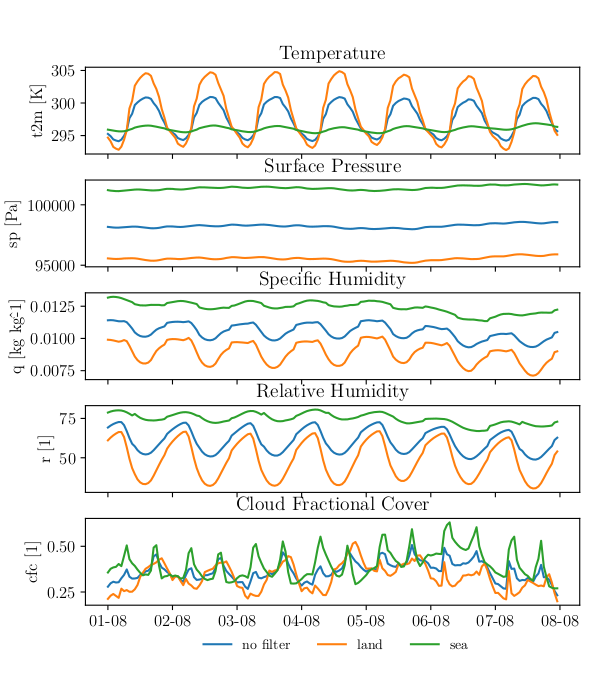
\includegraphics{python_figs/spatially_averaged_one_week_from_2012-08-01.png}
    \caption{Signal August 2012.}
    \label{fig:jan12}
\end{figure}

\begin{figure}[ht]
    \centering
    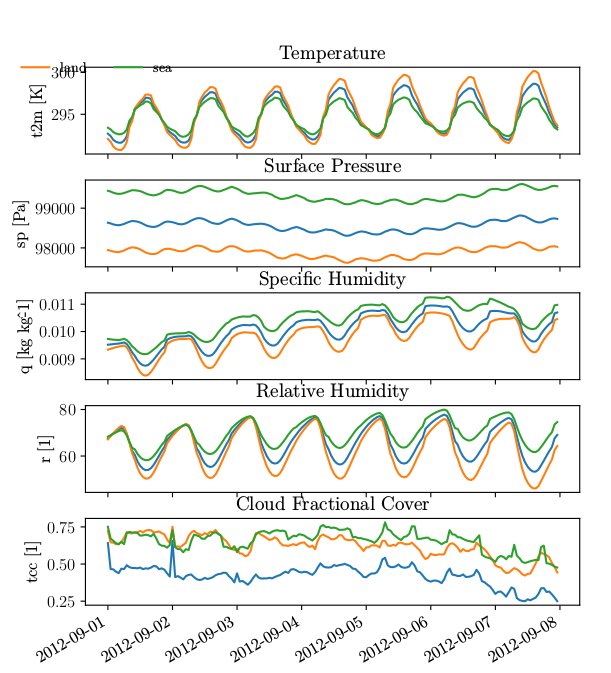
\includegraphics{python_figs/spatially_averaged_one_week_from_2012-09-01.png}
    \caption{Signal September 2012.}
    \label{fig:sep12}
\end{figure}


\begin{figure}[ht]
    \centering
    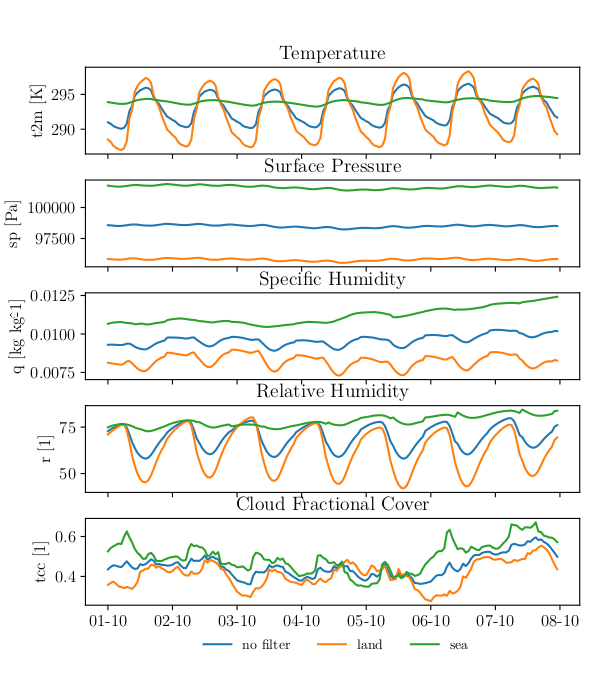
\includegraphics{python_figs/spatially_averaged_one_week_from_2012-10-01.png}
    \caption{Signal October 2012.}
    \label{fig:oct12}
\end{figure}


\begin{figure}[ht]
    \centering
    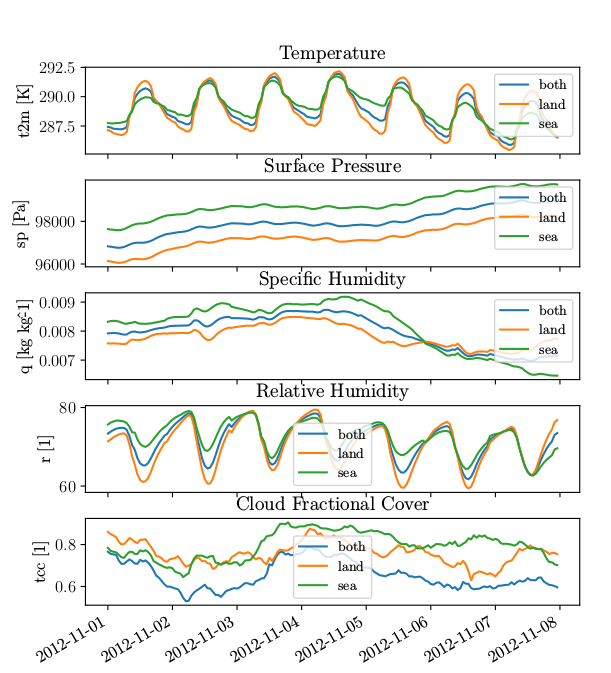
\includegraphics{python_figs/spatially_averaged_one_week_from_2012-11-01.png}
    \caption{Signal November 2012.}
    \label{fig:nov12}
\end{figure}

\begin{figure}[ht]
    \centering
    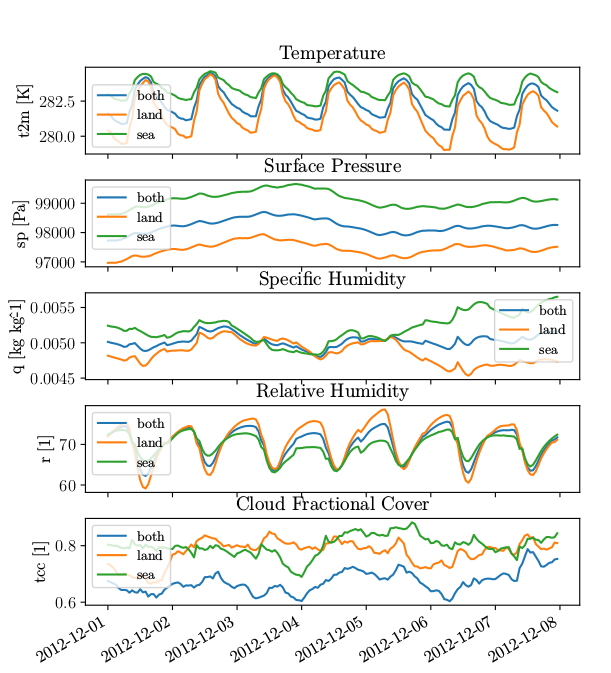
\includegraphics{python_figs/spatially_averaged_one_week_from_2012-12-01.png}
    \caption{Signal December 2012.}
    \label{fig:dec12}
\end{figure}


%%%%%%%%%%%%%%%%%%%%%%%%%%%%%%%%%%%%% signal artefact should be redefined if used 
\begin{figure}
    \centering
    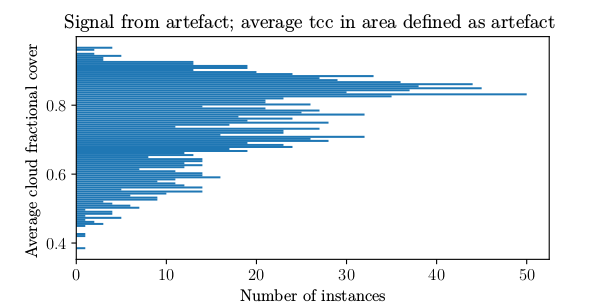
\includegraphics{python_figs/signal_artefact.png}
    \caption{Occurence of artefact, keep in mind that is not made any effort to distinguish this from when the entire area has cloud cover, this could be done by the ratio of artefact signal to land or something else. }
    \label{fig:signal_artefact}
\end{figure}


\chapter{Stuff I dont know if I should include.}
\tdplotsetmaincoords{60}{110}
%
\pgfmathsetmacro{\rvec}{1.6}
\pgfmathsetmacro{\thetavec}{30}
\pgfmathsetmacro{\phivec}{60}

\pgfmathsetmacro{\deltathetavec}{40}
\pgfmathsetmacro{\deltaphivec}{80}

\begin{figure}
    \centering
    
    
\tdplotsetmaincoords{60}{110}
%
\pgfmathsetmacro{\rvec}{1.0}

\pgfmathsetmacro{\thetavec}{30}
\pgfmathsetmacro{\deltathetavec}{40}
\pgfmathsetmacro{\deltatwothetavec}{50}
\pgfmathsetmacro{\deltathreethetavec}{60}

\pgfmathsetmacro{\phivec}{-30}
\pgfmathsetmacro{\deltaphivec}{10}
\pgfmathsetmacro{\deltatwophivec}{50}
\pgfmathsetmacro{\deltathreephivec}{90}

\begin{tikzpicture}[scale=5,tdplot_main_coords]

    %%%%%%%%%%%%%% Setting up axis and coordinate system.
    \coordinate (O) at (0,0,0); % origo
    \coordinate (z) at (0, 0, \rvec); % origo
    %\draw[thin, <->] (1, 0.7, 1.16) -- (1, 0.52, 1.2) node[pos = 0.8, above right]{\Large $d\theta$};
    \draw[very thick,->, opacity = 1.] (0,0,0) -- (1.7, 0, 0) node[anchor=north east]{\Large $x$};
    \draw[very thick,->,  opacity = 1.] (0,0,0) -- (0, 1.7, 0) node[anchor=north west]{\Large $y$};
    \draw[very thick,->,  opacity = 1.] (0,0,0) -- (0, 0, 1.7) node[anchor=south]{\Large $z$};
    \shade[ball color = teal, opacity = 0.1] (0,0,0) circle [radius=\rvec];
    \draw (0,0,0) circle [radius=\rvec];

    %%%%%%%%%%%%%%%%%%%%%%%%%%%% first column
    \tdplotsetcoord{P}{\rvec}{\thetavec}{\phivec}
    \tdplotsetcoord{dP}{\rvec}{\deltathetavec}{\phivec}
    \tdplotsetcoord{G}{\rvec}{\thetavec}{\deltaphivec}
    \tdplotsetcoord{dG}{\rvec}{\deltathetavec}{\deltaphivec}
    
    \draw[dashed, very thick, color=teal, fill = teal, opacity = 0.2] (P) -- (dP) -- (dG) -- (G) -- (P);
    \draw[dashed, very thick, color=teal] (P) -- (dP) -- (dG) -- (G) -- (P);
    
    \tdplotsetcoord{a}{\rvec}{\deltathetavec}{\phivec}
    \tdplotsetcoord{b}{\rvec}{\deltatwothetavec}{\phivec}
    \tdplotsetcoord{c}{\rvec}{\deltathetavec}{\deltaphivec}
    \tdplotsetcoord{d}{\rvec}{\deltatwothetavec}{\deltaphivec}
    
    \draw[dashed, very thick, color=teal, fill = teal, opacity = 0.2] (a) -- (b) -- (d)-- (c) -- (a);
    \draw[dashed, very thick, color=teal] (a) -- (b) -- (d)-- (c) -- (a);
    
    \tdplotsetcoord{e}{\rvec}{\deltatwothetavec}{\phivec}
    \tdplotsetcoord{f}{\rvec}{\deltathreethetavec}{\phivec}
    \tdplotsetcoord{g}{\rvec}{\deltatwothetavec}{\deltaphivec}
    \tdplotsetcoord{h}{\rvec}{\deltathreethetavec}{\deltaphivec}
    
    \draw[dashed, very thick, color=teal, fill = teal, opacity = 0.2] (e) -- (f) -- (h)-- (g) -- (e);
    \draw[dashed, very thick, color=teal] (e) -- (f) -- (h)-- (g) -- (e);

    %%%%%%%%%%%%%%%%%%%%%%%%%%%%%%%% second column
      
    \tdplotsetcoord{P}{\rvec}{\thetavec}{\deltaphivec}
    \tdplotsetcoord{dP}{\rvec}{\deltathetavec}{\deltaphivec}
    \tdplotsetcoord{G}{\rvec}{\thetavec}{\deltatwophivec}
    \tdplotsetcoord{dG}{\rvec}{\deltathetavec}{\deltatwophivec}
    
    \draw[dashed, very thick, color=teal, fill = teal, opacity = 0.2] (P) -- (dP) -- (dG) -- (G) -- (P);
    \draw[dashed, very thick, color=teal] (P) -- (dP) -- (dG) -- (G) -- (P);
  
      
    \tdplotsetcoord{a}{\rvec}{\deltathetavec}{\deltaphivec}
    \tdplotsetcoord{b}{\rvec}{\deltatwothetavec}{\deltaphivec}
    \tdplotsetcoord{c}{\rvec}{\deltathetavec}{\deltatwophivec}
    \tdplotsetcoord{d}{\rvec}{\deltatwothetavec}{\deltatwophivec}
    
    \draw[dashed, very thick, color=teal, fill = teal, opacity = 0.2] (a) -- (b) -- (d)-- (c) -- (a);
    \draw[dashed, very thick, color=teal] (a) -- (b) -- (d)-- (c) -- (a);
  
  
    \tdplotsetcoord{e}{\rvec}{\deltatwothetavec}{\deltaphivec}
    \tdplotsetcoord{f}{\rvec}{\deltathreethetavec}{\deltaphivec}
    \tdplotsetcoord{g}{\rvec}{\deltatwothetavec}{\deltatwophivec}
    \tdplotsetcoord{h}{\rvec}{\deltathreethetavec}{\deltatwophivec}
    
    \draw[dashed, very thick, color=teal, fill = teal, opacity = 0.2] (e) -- (f) -- (h)-- (g) -- (e);
    \draw[dashed, very thick, color=teal] (e) -- (f) -- (h)-- (g) -- (e);
    
    
    %%%%%%%%%%%%%%%%%%%%%%%%%%%%%%%% third column
    \tdplotsetcoord{P}{\rvec}{\thetavec}{\deltatwophivec}
    \tdplotsetcoord{dP}{\rvec}{\deltathetavec}{\deltatwophivec}
    \tdplotsetcoord{G}{\rvec}{\thetavec}{\deltathreephivec}
    \tdplotsetcoord{dG}{\rvec}{\deltathetavec}{\deltathreephivec}
    
    \draw[dashed, very thick, color=teal, fill = teal, opacity = 0.2] (P) -- (dP) -- (dG) -- (G) -- (P);
    \draw[dashed, very thick, color=teal] (P) -- (dP) -- (dG) -- (G) -- (P);
  
    \tdplotsetcoord{a}{\rvec}{\deltathetavec}{\deltatwophivec}
    \tdplotsetcoord{b}{\rvec}{\deltatwothetavec}{\deltatwophivec}
    \tdplotsetcoord{c}{\rvec}{\deltathetavec}{\deltathreephivec}
    \tdplotsetcoord{d}{\rvec}{\deltatwothetavec}{\deltathreephivec}
    
    \draw[dashed, very thick, color=teal, fill = teal, opacity = 0.2] (a) -- (b) -- (d)-- (c) -- (a);
    \draw[dashed, very thick, color=teal] (a) -- (b) -- (d)-- (c) -- (a);
  
    \tdplotsetcoord{e}{\rvec}{\deltatwothetavec}{\deltatwophivec}
    \tdplotsetcoord{f}{\rvec}{\deltathreethetavec}{\deltatwophivec}
    \tdplotsetcoord{g}{\rvec}{\deltatwothetavec}{\deltathreephivec}
    \tdplotsetcoord{h}{\rvec}{\deltathreethetavec}{\deltathreephivec}
    
    \draw[dashed, very thick, color=teal, fill = teal, opacity = 0.2] (e) -- (f) -- (h)-- (g) -- (e);
    \draw[dashed, very thick, color=teal] (e) -- (f) -- (h)-- (g) -- (e);
    
    %%%%%%%%%%%%%%%%%%%%%%%%%% Adding coordinate information

    % First column
    \draw[thick](0.3, -0.25, 0.5)node[scale=0.8, rotate = -15]{$(i,j-1)$};
    \draw[thick](0.3, -0.17, 0.7)node[scale=0.8, rotate = -15]{$(i+1,j-1)$};
    \draw[thick](0.3, -0.3, 0.3)node[scale=0.8, rotate = -15]{$(i-1,j-1)$};

    % Second column
    \draw[thick](0.5, 0.3, 0.65)node[scale=0.8, rotate = 5]{$(i,j)$};
    \draw[thick](0.5, 0.3, 0.85)node[scale=0.8, rotate = 5]{$(i+1,j)$};
    \draw[thick](0.5, 0.3, 0.45)node[scale=0.8, rotate = 5]{$(i-1,j)$};
    
    % Third column
    \draw[thick](0.5, 0.73, 0.87)node[scale=0.8, rotate = 35]{$(i,j+1)$};
    \draw[thick](0.5, 0.8, 0.7)node[scale=0.8, rotate = 35]{$(i-1,j+1)$};

    \draw[thick](0.05, 0.45, 0.73)node[scale=0.8, rotate = 35]{$(i+1,j+1)$};

    \tdplotsetthetaplanecoords{\phivec};
    \shade[ball color=teal,tdplot_screen_coords,opacity=0.2] (O) circle[radius=\rvec];
    \foreach \X/\Y in {xy/z,yz/x,zx/y}
        {\begin{scope}[canvas is \X\space plane at \Y=\rvec]
         \fill circle[radius=1pt];
        \end{scope}}
    \end{tikzpicture}
    
    \caption{Sketch illustrating the relative size of neighboring pixels in uniform grid of \acrshort{ecc}, projected onto spherical coordinates. The areas of pixels in a uniform grid decrease poleward.}
    \label{fig:relative_size_neigbouring_pixels}
\end{figure}
